\documentclass[tikz,border=6pt]{standalone}
\usepackage[T1]{fontenc}
\usepackage{tikz}
\usetikzlibrary{arrows.meta,positioning,fit}

\definecolor{panelblue}{HTML}{BFD8FF}
\definecolor{panelgreen}{HTML}{BFE8C8}
\definecolor{panelyellow}{HTML}{FFE09A}
\definecolor{panelred}{HTML}{EFB7B7}
\definecolor{panelgray}{HTML}{E1E5EA}
\definecolor{linegray}{HTML}{374151}
\definecolor{bboxfill}{HTML}{CFE1FF}
\definecolor{edgefill}{HTML}{FFD3A3}
\definecolor{motionfill}{HTML}{BFE8C8}
\definecolor{relationfill}{HTML}{FFE59E}

\tikzset{
  box/.style={draw=linegray, rounded corners=2pt, line width=0.8pt, align=center, font=\sffamily\small, inner sep=5pt},
  smallbox/.style={draw=linegray, rounded corners=2pt, line width=0.6pt, align=center, font=\sffamily\scriptsize, inner sep=3pt},
  arrow/.style={-Latex, line width=0.8pt, draw=linegray},
  trainarrow/.style={-Latex, line width=0.7pt, draw=linegray, dashed},
}

\begin{document}
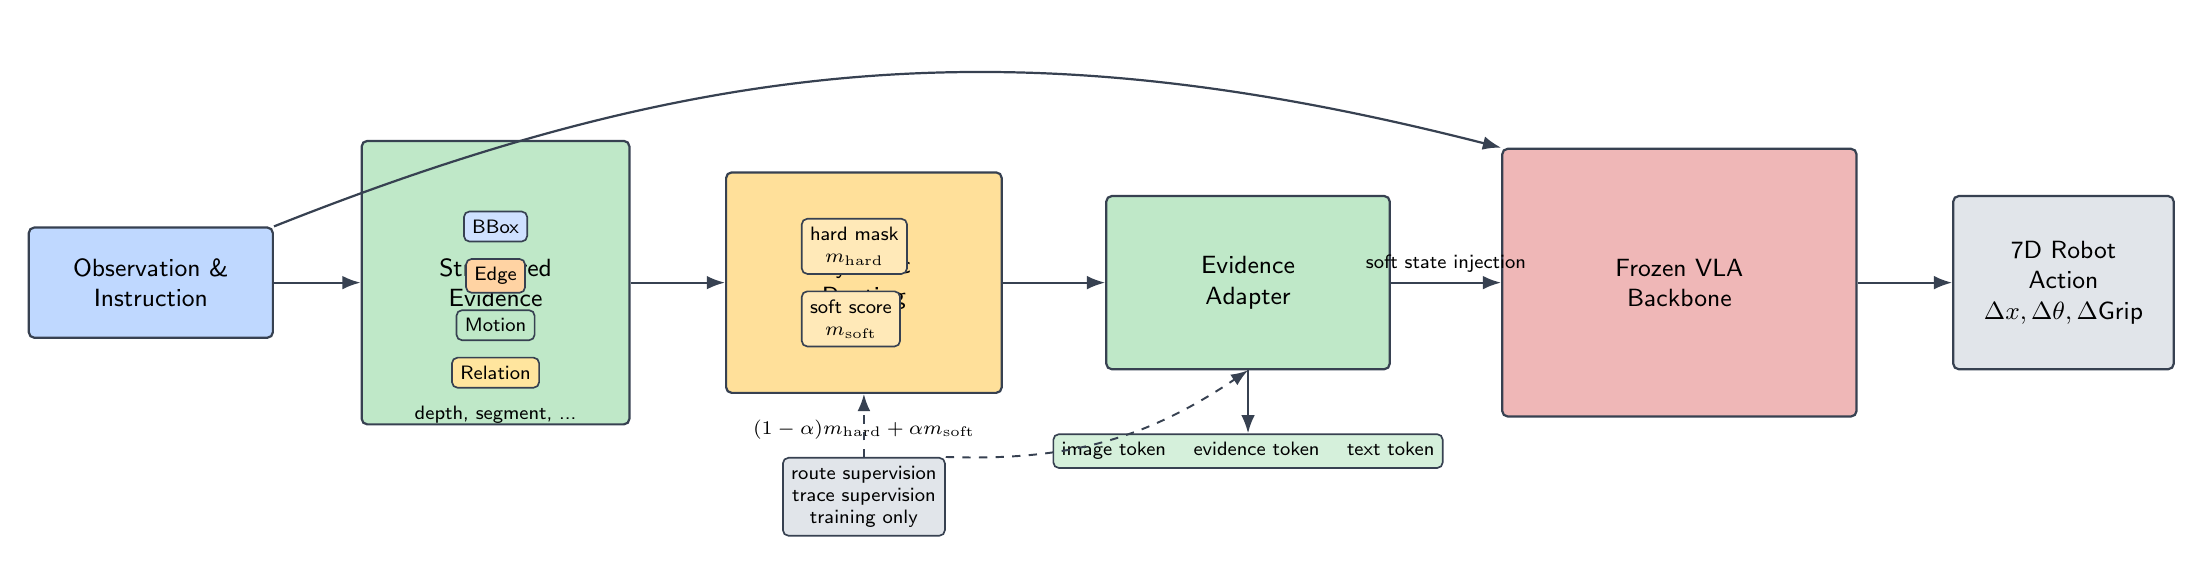
\begin{tikzpicture}[node distance=8mm and 10mm]

\node[box, fill=panelblue, minimum width=31mm, minimum height=14mm] (input)
  {Observation \&\\Instruction};

\node[box, fill=panelgreen, right=11mm of input, minimum width=34mm, minimum height=36mm] (evidence)
  {Structured\\Evidence};
\node[smallbox, fill=bboxfill, anchor=north] at ([yshift=-9mm]evidence.north) (bbox) {BBox};
\node[smallbox, fill=edgefill, below=2mm of bbox] (edge) {Edge};
\node[smallbox, fill=motionfill, below=2mm of edge] (motion) {Motion};
\node[smallbox, fill=relationfill, below=2mm of motion] (relation) {Relation};
\node[font=\sffamily\scriptsize, below=1mm of relation] (other) {depth, segment, ...};

\node[box, fill=panelyellow, right=12mm of evidence, minimum width=35mm, minimum height=28mm] (router)
  {Dynamic\\Routing};
\node[smallbox, fill=panelyellow!70!white, above right=1mm and -8mm of router.center] (hard) {hard mask\\$m_{\mathrm{hard}}$};
\node[smallbox, fill=panelyellow!70!white, below right=1mm and -8mm of router.center] (soft) {soft score\\$m_{\mathrm{soft}}$};
\node[font=\sffamily\scriptsize, below=2mm of router] (blend)
  {$(1-\alpha)m_{\mathrm{hard}}+\alpha m_{\mathrm{soft}}$};

\node[box, fill=panelgreen, right=13mm of router, minimum width=36mm, minimum height=22mm] (adapter)
  {Evidence\\Adapter};

\node[box, fill=panelred, right=14mm of adapter, minimum width=45mm, minimum height=34mm] (vla)
  {Frozen VLA\\Backbone};

\node[box, fill=panelgray, right=12mm of vla, minimum width=28mm, minimum height=22mm] (action)
  {7D Robot\\Action\\$\Delta x,\Delta \theta,\Delta$Grip};

\node[smallbox, fill=panelgreen!65!white, below=8mm of adapter] (tokens)
  {image token \quad evidence token \quad text token};

\node[smallbox, fill=panelgray, below=8mm of router] (trace)
  {route supervision\\trace supervision\\training only};

\draw[arrow] (input) -- (evidence);
\draw[arrow] (evidence) -- (router);
\draw[arrow] (router) -- (adapter);
\draw[arrow] (adapter) -- node[above, font=\sffamily\scriptsize]{soft state injection} (vla);
\draw[arrow] (input.north east) to[bend left=18] (vla.north west);
\draw[arrow] (vla) -- (action);

\draw[trainarrow] (trace.north) -- (router.south);
\draw[trainarrow] (trace.north east) to[bend right=18] (adapter.south);
\draw[arrow] (adapter.south) -- (tokens.north);

\end{tikzpicture}
\end{document}
